\chapter{NAND, NOR gates}
%\ref{sec:background}.

\section{Aim}
%\label{sec:objectives}
	To verify and interpret the logic and truth table for NAND, NOR gates using Resistor Transistor Logic (RTL)

\section{Apparatus}
%\label{sec:objectives}
	\begin{itemize}
		\tightlist
		\item Kit for realization of gates
		\item Connecting Leads
	\end{itemize}

\section{Circuits}
	

\section{Theory}
	Logic gates are the basic building blocks of any digital system. Logic gates are electronic circuits having one or more than one input and only one output. The relationship between the input and the output is based on a certain logic. Based on this, logic gates are named as:
	\begin{enumerate}
		\tightlist
		\item AND gate
		\item OR gate
		\item NOT gate
		\item NAND gate
		\item NOT gate
		\item Ex-OR gate
		\item Ex-NOR gate
	\end{enumerate}
	
	\subsection{NAND gate}
	This is a NOT-AND gate which is equal to an AND gate followed by a NOT gate. The outputs of all NAND gates are high if any of the inputs are low. The symbol is an AND gate with a small circle on the output. The small circle represents inversion.
	\begin{align*}
		Y &= \overline{A . B}
	\end{align*}
	A simple 2-input logic NAND gate can be constructed using RTL (Resistor-transistor-logic) switches connected together as shown in Figure \ref{fig:nand_circuit} with the inputs connected directly to the transistor bases. Either transistor must be cut-off or “OFF” for an output at Q.
	\begin{figure}[ht]
		\centering 
		\subfloat[Symbol]
		{
			\begin{circuitikz} \draw
				(0,0) node[nand port] (myand1) {}
				(myand1.in 1) node[anchor=east] {A}
				(myand1.in 2) node[anchor=east] {B}
				(myand1.out) node[anchor=west] {Y}
				;
			\end{circuitikz}
			\label{fig:nand_symbol}
		}	
		\hfill
		\subfloat[Truth Table]
		{
			\begin{tabular}{|c|c|c|}
				\hline
				\multicolumn{2}{|c|}{Input} & Output \\
				\hline
				$A$ & $B$ & $Y=\overline{A.B}$ \\
				\hline
				0 & 0 & 1 \\
				\hline
				0 & 1 & 1 \\
				\hline
				1 & 0 & 1 \\
				\hline
				1 & 1 & 0 \\
				\hline
			\end{tabular}
			\label{fig:nand_table}
		}
		\hfill
		\subfloat[RTL Design]{
			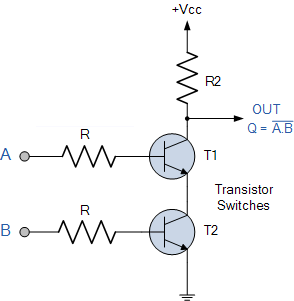
\includegraphics[width=0.25\textwidth,valign=c]{img/exp2/fig1}
			\label{fig:nand_circuit}
		}
		\caption{\textit{NAND gate}}
	\end{figure}
	
	
	\subsection{NOR gate}
		This is a NOT-OR gate which is equal to an OR gate followed by a NOT gate. The outputs of all NOR gates are low if any of the inputs are high. The symbol is an OR gate with a small circle on the output. The small circle represents inversion.
		\begin{align*}
			Y &= \overline{A + B}
		\end{align*}		
		A simple 2-input logic NOR gate can be constructed using RTL (Resistor-transistor-logic) switches connected together as shown in Figure \ref{fig:nor_circuit} with the inputs connected directly to the transistor bases. Both transistors must be cut-off or “OFF” for an output at Q.
		\begin{figure}[ht]
			\centering 
			\subfloat[Symbol]
			{
				\begin{circuitikz} \draw
					(0,0) node[nor port] (myand1) {}
					(myand1.in 1) node[anchor=east] {A}
					(myand1.in 2) node[anchor=east] {B}
					(myand1.out) node[anchor=west] {Y}
					;
				\end{circuitikz}
				\label{fig:nor_symbol}
			}	
			\hfill
			\subfloat[Truth Table]
			{
				\begin{tabular}{|c|c|c|}
					\hline
					\multicolumn{2}{|c|}{Input} & Output \\
					\hline
					$A$ & $B$ & $Y=\overline{A+B}$ \\
					\hline
					0 & 0 & 1 \\
					\hline
					0 & 1 & 0 \\
					\hline
					1 & 0 & 0 \\
					\hline
					1 & 1 & 0 \\
					\hline
				\end{tabular}
				\label{fig:nor_table}
			}
			\hfill
			\subfloat[RTL Design]{
				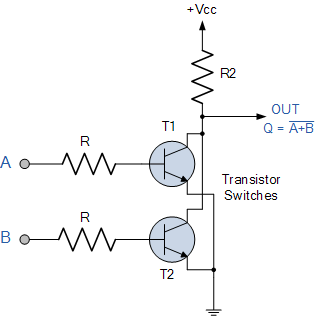
\includegraphics[width=0.25\textwidth,valign=c]{img/exp2/fig2}
				\label{fig:nor_circuit}
			}
			\caption{\textit{NOR gate}}
		\end{figure}
		
\section{Procedure}
	\subsection{NAND gate}
		\begin{figure}[ht]
			\centering 
			\subfloat[Simulator 1]{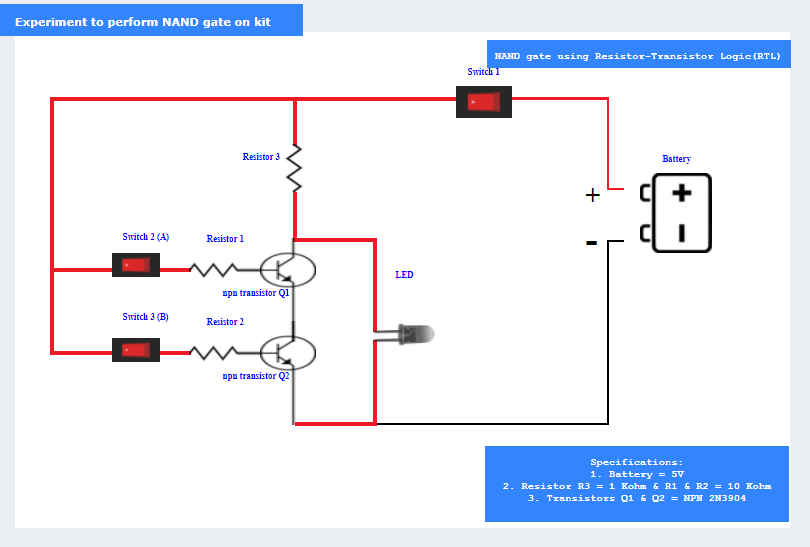
\includegraphics[width=0.45\textwidth,valign=c]{img/exp2/fig3}
				\label{fig:nand_sim:1}}	
			\hfill
			\subfloat[Simulator 2]{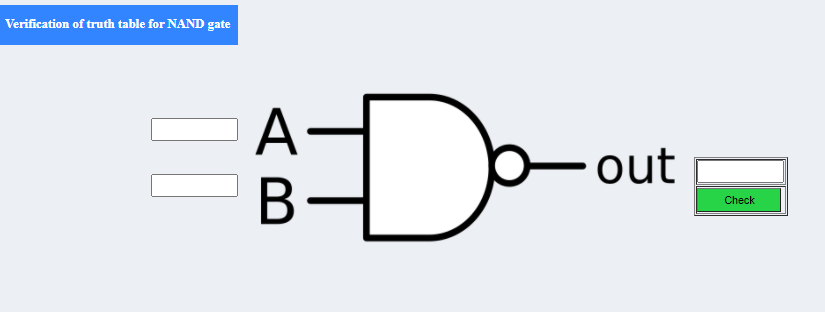
\includegraphics[width=0.4\textwidth,valign=c]{img/exp2/fig4}
				\label{fig:nand_sim:2}}			
			\caption{\textit{Simulator for realizing circuit for NAND gate}}
		\end{figure}
		\subsubsection{Simulator 1}
			\begin{enumerate}
				\tightlist
				\item Connect the supply(+5V) to the circuit.
				\item Press the switches for inputs "A" and "B".			
				\item The bulb glows if any one or both the switches are OFF else it won't glow.
				\item Repeat step-2 and step-3 for all state of inputs.
			\end{enumerate}
		\subsubsection{Simulator 2}
			\begin{enumerate}
				\tightlist
				\item Enter the Boolean input "A" and "B".
				\item Enter the Boolean output for your corresponding inputs.
				\item Click on "Check" Button to verify your output.			
			\end{enumerate}	

	\subsection{NOR gate}
		\begin{figure}[ht]
			\centering 
			\subfloat[Simulator 1]{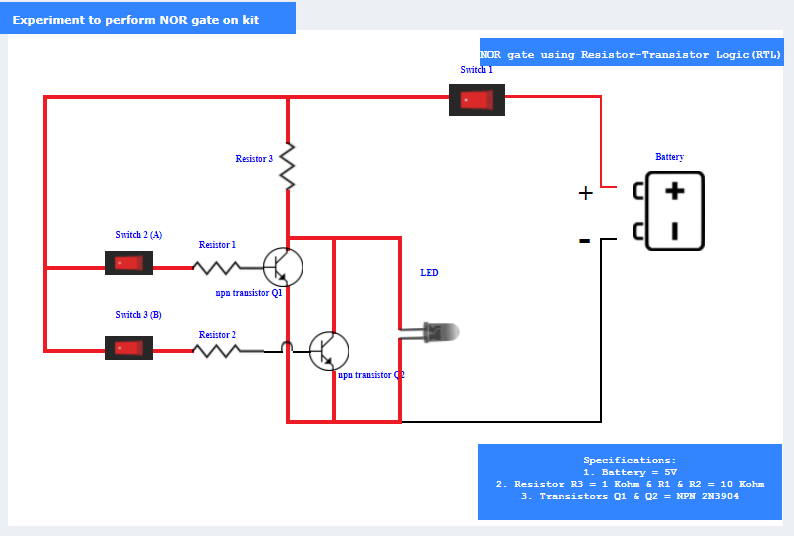
\includegraphics[width=0.45\textwidth,valign=c]{img/exp2/fig5}
				\label{fig:nor_sim:1}}	
			\hfill
			\subfloat[Simulator 2]{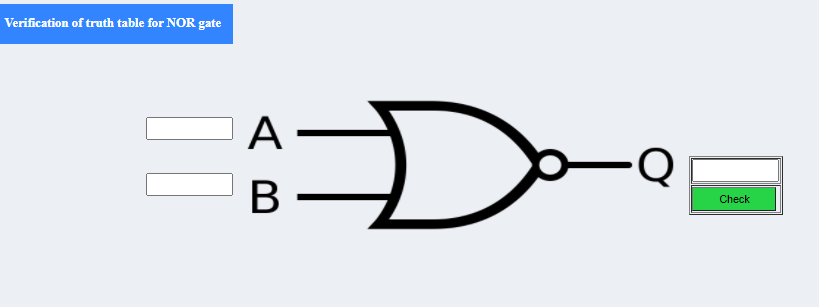
\includegraphics[width=0.4\textwidth,valign=c]{img/exp2/fig6}
				\label{fig:nor_sim:2}}
			\caption{\textit{Simulator for realizing circuit for NOR gate}}
		\end{figure}
		\subsubsection{Simulator 1}
			\begin{enumerate}
				\tightlist
				\item Connect the supply(+5V) to the circuit.
				\item Press the switches for inputs "A" and "B".			
				\item The bulb glows if both the switches are OFF else it won't glow.
				\item Repeat step-2 and step-3 for all state of inputs.
			\end{enumerate}
		\subsubsection{Simulator 2}
			\begin{enumerate}
				\tightlist
				\item Enter the Boolean input "A" and "B".
				\item Enter the Boolean output for your corresponding inputs.
				\item Click on "Check" Button to verify your output.			
			\end{enumerate}

\section{Observations}
	\subsection{NAND gate}
			\begin{figure}[ht]
				\centering 
				\subfloat[Either of the Inputs OFF, LED is ON]{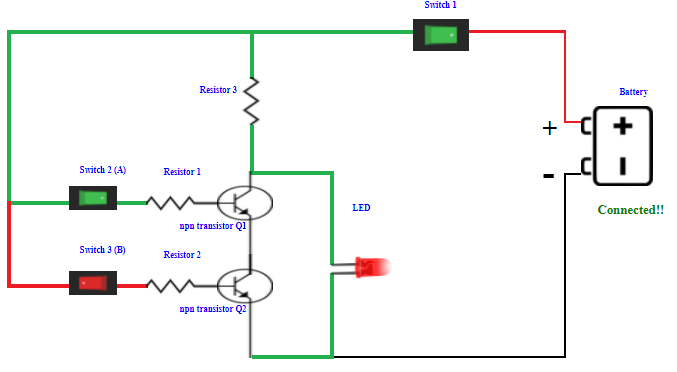
\includegraphics[width=0.45\textwidth,valign=c]{img/exp2/fig7}
					\label{fig:nand_obs:1}}	
				\hfill
				\subfloat[Both Inputs ON, LED is OFF]{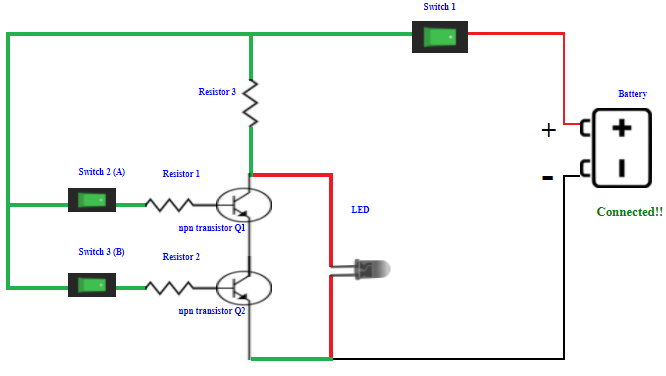
\includegraphics[width=0.45\textwidth,valign=c]{img/exp2/fig8}
					\label{fig:nand_obs:2}}			
				\caption{\textit{Observations for different Input Values}}
			\end{figure}
			\begin{figure}[h]
				\centering
				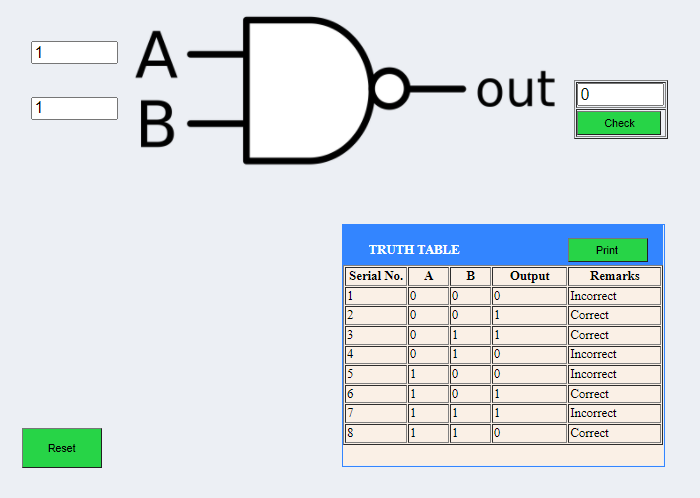
\includegraphics[width=0.85\linewidth]{img/exp2/fig9}
				\caption{\textit{Observations for verification of Truth Table of the NAND gate}}
				\label{fig:nand_obs_2}
			\end{figure}

\pagebreak
	\subsection{NOR gate}
			\begin{figure}[ht]
				\centering 
				\subfloat[Either of the Inputs ON, LED is OFF]{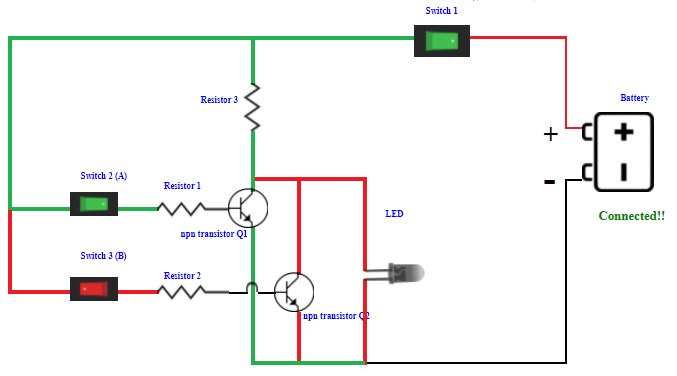
\includegraphics[width=0.45\textwidth,valign=c]{img/exp2/fig10}
					\label{fig:nor_obs:1}}	
				\hfill
				\subfloat[Both Inputs OFF, LED is ON]{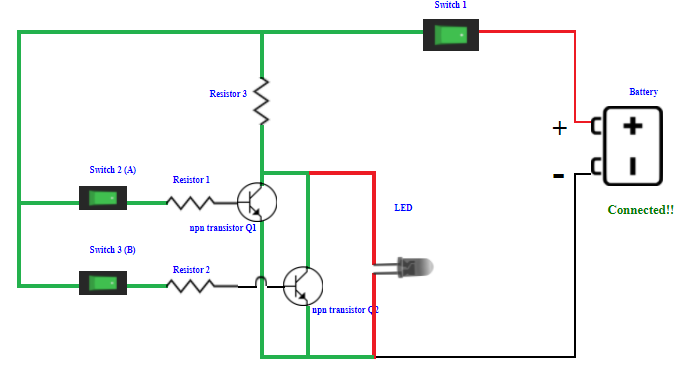
\includegraphics[width=0.45\textwidth,valign=c]{img/exp2/fig11}
					\label{fig:nor_obs:2}}
				\caption{\textit{Observations for different Input Values}}
			\end{figure}
			\begin{figure}[h]
				\centering
				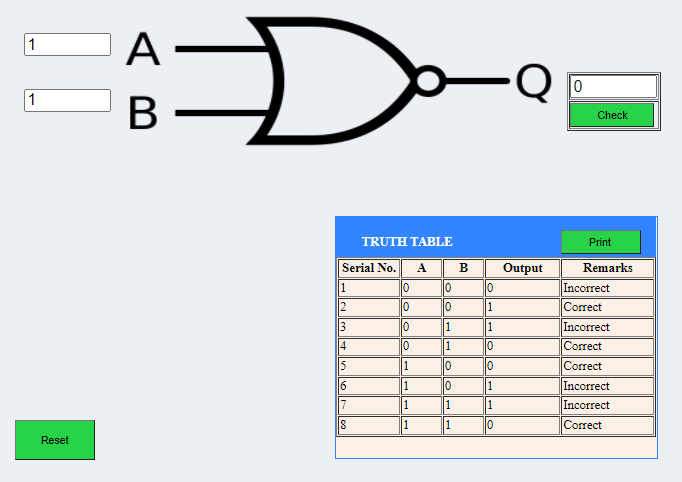
\includegraphics[width=0.85\linewidth]{img/exp2/fig12}
				\caption{\textit{Observations for verification of Truth Table of the NOR gate}}
				\label{fig:nor_obs_2}
			\end{figure}
			
\section{Precautions}
	\begin{enumerate}
		\tightlist
		\item Make the connections when power supply is OFF.
		\item Ensure that the connections are tight.
		\item Change the status of inputs only when power supply is OFF.
	\end{enumerate}